\documentclass[11pt,a4paper]{article}

% ---------------------------------------------------------------- packages
\usepackage[margin=1in]{geometry}
\usepackage[T1]{fontenc}
\usepackage{lmodern}
\usepackage{microtype}
\usepackage{amsmath,amssymb,amsthm,mathtools}
\usepackage{booktabs}
\usepackage{graphicx}
\usepackage{xcolor}
\usepackage{enumitem}
\usepackage[skins,breakable]{tcolorbox}
\usepackage{caption}
\usepackage[colorlinks=true,linkcolor=blue!50!black,citecolor=blue!50!black,urlcolor=blue!50!black]{hyperref}

\captionsetup{font=small,labelfont=bf}
\setlist{itemsep=2pt,topsep=4pt}
\setlength{\parskip}{4pt}
\setlength{\parindent}{0pt}

% ---------------------------------------------------------------- notation
\newcommand{\Prob}{\mathbb{P}}
\newcommand{\Ex}{\mathbb{E}}
\DeclareMathOperator{\TPR}{TPR}
\DeclareMathOperator{\FPR}{FPR}
\DeclareMathOperator{\TNR}{TNR}
\DeclareMathOperator{\FNR}{FNR}
\DeclareMathOperator{\Prec}{Prec}
\DeclareMathOperator{\Rec}{Rec}
\DeclareMathOperator{\AUROC}{AUC\text{-}ROC}
\DeclareMathOperator{\AP}{AP}
\newcommand{\Fone}{F_{1}}

% ---------------------------------------------------------------- theorems
\theoremstyle{plain}
\newtheorem{theorem}{Theorem}
\newtheorem{proposition}[theorem]{Proposition}
\newtheorem{lemma}[theorem]{Lemma}
\newtheorem{corollary}[theorem]{Corollary}
\theoremstyle{definition}
\newtheorem{definition}[theorem]{Definition}
\newtheorem{example}[theorem]{Example}
\theoremstyle{remark}
\newtheorem*{remark}{Remark}

% ---------------------------------------------------------------- boxes
\newtcolorbox{metric}[1]{
  enhanced, breakable, colback=blue!3!white, colframe=blue!55!black,
  boxrule=0.5pt, arc=2pt, left=6pt, right=6pt, top=4pt, bottom=4pt,
  title={#1}, fonttitle=\bfseries\small, coltitle=black, colbacktitle=blue!10!white
}
\newtcolorbox{insight}[1][Key idea]{
  enhanced, breakable, colback=orange!5!white, colframe=orange!70!black,
  boxrule=0.5pt, arc=2pt, left=6pt, right=6pt, top=4pt, bottom=4pt,
  title={#1}, fonttitle=\bfseries\small, coltitle=black, colbacktitle=orange!15!white
}

\title{Evaluating Binary Classifiers under Class Imbalance:\\
ROC-AUC, AUC-PR (Average Precision) and the $F_1$ score}
\author{}
\date{\today}

\begin{document}
\maketitle

\begin{abstract}
\noindent
These notes build up the standard evaluation metrics for binary classification from the confusion
matrix, define the two threshold-free summaries ROC-AUC and AUC-PR, illustrate them with worked
examples and plots, and then prove why AUC-PR is the more informative of the two when the positive
class is rare. The thread running through everything is a single identity,
$\Prec = \TPR/(\TPR + k\,\FPR)$, where $k$ is the number of negatives per positive.
\end{abstract}

\tableofcontents

% =====================================================================
\section{Classification basics}
% =====================================================================

\subsection{Setup and notation}
We consider binary classification with a label $Y\in\{0,1\}$, where $1$ is the \emph{positive} class
(e.g.\ a fraudulent transaction) and $0$ the \emph{negative} class. A model produces a real-valued
\emph{score} $S=s(X)$, higher meaning ``more likely positive''. A threshold $t$ turns the score into a
decision
\[
  \hat Y_t \;=\; \mathbf 1\{S>t\}.
\]
Let $P$ and $N$ be the numbers of positive and negative cases and $n=P+N$. Two quantities describe
how imbalanced the data are:
\[
  \pi \;=\; \frac{P}{n}\quad\text{(prevalence)},
  \qquad
  k \;=\; \frac{N}{P} \;=\; \frac{1-\pi}{\pi}\quad\text{(class ratio: negatives per positive)}.
\]
For a fraud rate of $0.1\%$ we have $\pi=0.001$ and $k=999$. Finally, $S^{+}$ and $S^{-}$ denote the score
of a randomly drawn positive and negative case respectively; their distributions are the
\emph{class-conditional score distributions}.

\subsection{The confusion matrix}
Fixing a threshold $t$, every case falls into exactly one cell:

\begin{center}
\begin{tabular}{lcc}
\toprule
 & Predicted positive & Predicted negative \\
\midrule
Actual positive ($P$ cases) & TP (true positive)  & FN (false negative) \\
Actual negative ($N$ cases) & FP (false positive) & TN (true negative)  \\
\bottomrule
\end{tabular}
\end{center}
so that $\mathrm{TP}+\mathrm{FN}=P$ and $\mathrm{FP}+\mathrm{TN}=N$. Everything below is a function of
these four counts.

\subsection{Rates conditioned on the true class}
The first four metrics divide by a \emph{row total} of the confusion matrix. Each is therefore a
conditional probability given the true class, which is why none of them depends on $\pi$.

\begin{metric}{True positive rate (TPR)}
Also known as \textbf{recall}, \textbf{sensitivity}, \textbf{hit rate}, detection rate, or
\textbf{power} ($=1-$ Type~II error rate). It is the probability or proportion of actual positive cases
that are correctly flagged as positive.
\[
  \TPR \;=\; \Rec \;=\; \frac{\mathrm{TP}}{\mathrm{TP}+\mathrm{FN}} \;=\; \frac{\mathrm{TP}}{P}
  \;=\; \Prob(\hat Y_t=1\mid Y=1) \;=\; \Prob(S^{+}>t).
\]
\end{metric}

\begin{metric}{False negative rate (FNR)}
Also known as the \textbf{miss rate} or \textbf{Type~II error rate}. It is the proportion of actual
positive cases that are missed.
\[
  \FNR \;=\; \frac{\mathrm{FN}}{\mathrm{FN}+\mathrm{TP}} \;=\; 1-\TPR \;=\; \Prob(S^{+}\le t).
\]
\end{metric}

\begin{metric}{False positive rate (FPR)}
The false positive rate (FPR)---also known as \textbf{fall-out}, \textbf{false alarm rate}, or
\textbf{Type~I error rate}---is the probability or proportion of actual negative cases that are
incorrectly flagged as positive.
\[
  \FPR \;=\; \frac{\mathrm{FP}}{\mathrm{FP}+\mathrm{TN}} \;=\; \frac{\mathrm{FP}}{N}
  \;=\; \Prob(\hat Y_t=1\mid Y=0) \;=\; \Prob(S^{-}>t).
\]
\end{metric}

\begin{metric}{True negative rate (TNR)}
Also known as \textbf{specificity} or \textbf{selectivity}. It is the proportion of actual negative cases
correctly left unflagged.
\[
  \TNR \;=\; \frac{\mathrm{TN}}{\mathrm{TN}+\mathrm{FP}} \;=\; 1-\FPR \;=\; \Prob(S^{-}\le t).
\]
\end{metric}

\subsection{Rates conditioned on the prediction}
The next three metrics divide by a \emph{column total}: they answer ``given that the model said
positive (negative), how often is it right?''. They mix the two classes in the proportion
$P:N$, so they \emph{do} depend on $\pi$.

\begin{metric}{Precision (positive predictive value, PPV)}
The proportion of flagged cases that are truly positive. Its complement is the
\textbf{false discovery rate}, $\mathrm{FDR}=1-\Prec$: the share of alerts that are false alarms.
\[
  \Prec \;=\; \frac{\mathrm{TP}}{\mathrm{TP}+\mathrm{FP}} \;=\; \Prob(Y=1\mid \hat Y_t=1).
\]
\end{metric}

\begin{metric}{Negative predictive value (NPV)}
The proportion of unflagged cases that are truly negative.
\[
  \mathrm{NPV} \;=\; \frac{\mathrm{TN}}{\mathrm{TN}+\mathrm{FN}} \;=\; \Prob(Y=0\mid \hat Y_t=0).
\]
\end{metric}

\subsection{Single-number summaries at one threshold}

\begin{metric}{Accuracy and balanced accuracy}
\[
  \mathrm{Acc} \;=\; \frac{\mathrm{TP}+\mathrm{TN}}{n} \;=\; \pi\,\TPR + (1-\pi)\,\TNR,
  \qquad
  \mathrm{BalAcc} \;=\; \tfrac12(\TPR+\TNR).
\]
Accuracy weights the two classes by their frequency, so under heavy imbalance it is dominated by the
majority class (the \emph{accuracy paradox}: with $\pi=0.001$, a model that never flags anything has
$\mathrm{Acc}=99.9\%$ and $\TPR=0$). Balanced accuracy removes the dependence on $\pi$ by
weighting both classes equally.
\end{metric}

\begin{metric}{$F_1$ and $F_\beta$ scores}
$F_1$ is the \textbf{harmonic mean} of precision and recall at a single threshold:
\[
  \Fone \;=\; \frac{2\,\Prec\cdot\Rec}{\Prec+\Rec} \;=\; \frac{2\,\mathrm{TP}}{2\,\mathrm{TP}+\mathrm{FP}+\mathrm{FN}}.
\]
The harmonic mean punishes imbalance between the two: $\Prec=1$ with $\Rec=0.01$ gives
$\Fone\approx0.02$, not $0.5$. The general form
$F_\beta=\dfrac{(1+\beta^2)\,\Prec\cdot\Rec}{\beta^2\,\Prec+\Rec}$ treats recall as $\beta$ times as
important as precision, so $\beta>1$ favours recall. Like precision, $F_\beta$ ignores true negatives.
\end{metric}

\begin{metric}{Matthews correlation coefficient (MCC)}
The correlation between prediction and truth, using all four cells:
\[
  \mathrm{MCC} \;=\; \frac{\mathrm{TP}\cdot\mathrm{TN}-\mathrm{FP}\cdot\mathrm{FN}}
  {\sqrt{(\mathrm{TP}+\mathrm{FP})(\mathrm{TP}+\mathrm{FN})(\mathrm{TN}+\mathrm{FP})(\mathrm{TN}+\mathrm{FN})}}\in[-1,1].
\]
\end{metric}

\subsection{The bridge identity: how \texorpdfstring{$\pi$}{the prevalence} enters}

The two families above are linked by the class ratio $k=N/P$. This is the single most important
identity in these notes.

\begin{proposition}[Prevalence enters through $k$]\label{prop:bridge}
For every threshold $t$,
\[
  \Prec \;=\; \frac{\TPR}{\TPR + k\,\FPR},
  \qquad
  \Fone \;=\; \frac{2\,\TPR}{1+\TPR+k\,\FPR},
  \qquad
  \mathrm{Acc} \;=\; \pi\,\TPR+(1-\pi)(1-\FPR).
\]
\end{proposition}
\begin{proof}
By definition $\mathrm{TP}=P\cdot\TPR$ and $\mathrm{FP}=N\cdot\FPR$. Hence
\[
  \Prec=\frac{P\,\TPR}{P\,\TPR+N\,\FPR}=\frac{\TPR}{\TPR+k\,\FPR}.
\]
For $F_1$, note $2\mathrm{TP}+\mathrm{FP}+\mathrm{FN} = 2P\,\TPR+N\,\FPR+P(1-\TPR)=P(1+\TPR+k\,\FPR)$,
so $\Fone = 2P\,\TPR/\big(P(1+\TPR+k\,\FPR)\big)$. The accuracy formula was shown above.
\end{proof}

Read this identity slowly: $\TPR$ and $\FPR$ are properties of the classifier alone (they are
conditional on the class), while $k$ is a property of the dataset. Whenever $k$ is large, even a tiny
$\FPR$ is multiplied by a huge number inside the denominator of precision.

\begin{table}[h]
\centering
\small
\caption{Which metrics depend on the class balance.}
\begin{tabular}{@{}lccc@{}}
\toprule
Metric & Conditions on & Uses TN? & Depends on $\pi$? \\
\midrule
TPR (recall), FNR & true class & no  & no \\
FPR, TNR          & true class & yes & no \\
Precision, FDR    & prediction & no  & \textbf{yes} \\
NPV               & prediction & yes & yes \\
Accuracy          & both       & yes & yes \\
Balanced accuracy & true class & yes & no \\
$F_1$, $F_\beta$  & both       & no  & \textbf{yes} \\
\bottomrule
\end{tabular}
\end{table}

% =====================================================================
\section{Threshold-free summaries: ROC-AUC and AUC-PR}
% =====================================================================

All the metrics so far describe one threshold $t$. As $t$ sweeps from $+\infty$ down to $-\infty$,
the classifier flags more and more cases and $(\FPR,\TPR)$ moves from $(0,0)$ to $(1,1)$. Tracing
this path under two different choices of axes gives the two curves.

\subsection{The ROC curve and ROC-AUC}

\begin{definition}[ROC curve]
The \emph{receiver operating characteristic} curve is the set of points
$\big(\FPR(t),\TPR(t)\big)$ over all thresholds $t$.
\end{definition}

A random classifier traces the diagonal $\TPR=\FPR$; a perfect one passes through the corner $(0,1)$. The
curve is unchanged by any strictly increasing transformation of the scores, since only the \emph{ranking}
matters.

\begin{definition}[ROC-AUC]
\[
  \AUROC \;=\; \int_0^1 \TPR\; d\FPR.
\]
\end{definition}

\begin{theorem}[Probabilistic interpretation]\label{thm:auc}
\[
  \AUROC \;=\; \Prob(S^{+}>S^{-}) + \tfrac12\,\Prob(S^{+}=S^{-}),
\]
the probability that a randomly chosen positive case is scored above a randomly chosen negative case.
\end{theorem}
\begin{proof}
Assume continuous scores with density $f^{-}$ for negatives (ties then have probability zero). Since
$\FPR(t)=\Prob(S^{-}>t)$, we have $d\FPR=-f^{-}(t)\,dt$, and as $t$ runs from $+\infty$ to $-\infty$ the
FPR runs from $0$ to $1$. Therefore
\[
  \AUROC=\int_{-\infty}^{\infty}\Prob(S^{+}>t)\,f^{-}(t)\,dt=\Prob(S^{+}>S^{-}).
\]
Ties contribute half by the usual trapezoid convention.
\end{proof}

So $\AUROC=0.5$ means random ranking and $1$ means every positive is ranked above every negative.
Note what does \emph{not} appear in this definition: the proportion of positives.

\subsection{The precision--recall curve and AUC-PR}

\begin{definition}[PR curve]
The \emph{precision--recall} curve is the set of points $\big(\Rec(t),\Prec(t)\big)=\big(\TPR(t),\Prec(t)\big)$
over all thresholds $t$.
\end{definition}

A classifier with no skill (scores independent of the label) has $\Prec=\pi$ at every recall level, so
the PR curve's baseline is the horizontal line at the \emph{prevalence}, not at $0.5$. True negatives
never appear on either axis.

\begin{definition}[AUC-PR\,/\,average precision]
Sort cases by decreasing score and let $\Prec_j,\Rec_j$ be the precision and recall after the $j$-th
distinct threshold (with $\Rec_0=0$). The \emph{average precision} is
\[
  \AP \;=\; \sum_{j}\big(\Rec_j-\Rec_{j-1}\big)\,\Prec_j
  \;\xrightarrow{\;\text{continuous limit}\;}\;
  \int_0^1 \Prec\; d\Rec .
\]
Equivalently, $\AP$ is the mean, over the $P$ positive cases, of the precision measured at the rank of
that positive.
\end{definition}

\begin{remark}
``Average precision'' is a recall-weighted average (weights $\Rec_j-\Rec_{j-1}$), not a plain average over
thresholds. ``AUC-PR'' is used loosely: computing the area with the trapezoid rule instead of this
step sum linearly interpolates between operating points, which is generally over-optimistic, and some
benchmarks use an ``interpolated'' variant. Always state which one you report. The step-wise
$\AP$ is what \texttt{sklearn.metrics.average\_precision\_score} computes.
\end{remark}

\begin{figure}[t]
\centering
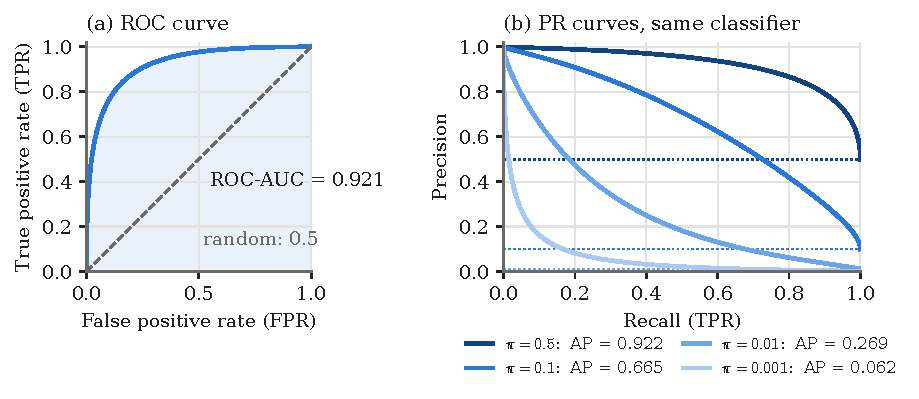
\includegraphics[width=\linewidth]{figs/fig_curves.pdf}
\caption{(a) ROC curve of a classifier whose scores are $\mathcal N(0,1)$ for negatives and
$\mathcal N(2,1)$ for positives; $\AUROC=\Phi(2/\sqrt2)\approx0.921$. (b) PR curves of \emph{the very
same classifier} when the prevalence is $\pi=0.5,0.1,0.01,0.001$. Dotted lines are the no-skill
baselines. The ROC curve does not move; the PR curve collapses toward zero.}
\label{fig:curves}
\end{figure}

Figure~\ref{fig:curves} already contains the whole story: one classifier, one ROC curve, but a
family of PR curves indexed by $\pi$. Sections~3 and~4 make this precise.

% =====================================================================
\section{Worked examples}
% =====================================================================

\subsection{A ten-transaction toy example}
Rank ten transactions by model score from highest to lowest. Three are fraud (P), seven are legitimate
(N), and the true labels in rank order are
\[
  \text{P, N, P, N, N, P, N, N, N, N}.
\]
Flagging the top $j$ cases gives the operating points in Table~\ref{tab:toy}.

\begin{table}[h]
\centering
\small
\caption{Operating points when flagging the top $j$ cases ($P=3$, $N=7$).}
\label{tab:toy}
\begin{tabular}{@{}cc cc cc cc@{}}
\toprule
$j$ & label & TP & FP & TPR (recall) & FPR & Precision \\
\midrule
1  & P & 1 & 0 & $1/3$ & $0$   & $1$ \\
2  & N & 1 & 1 & $1/3$ & $1/7$ & $1/2$ \\
3  & P & 2 & 1 & $2/3$ & $1/7$ & $2/3$ \\
4  & N & 2 & 2 & $2/3$ & $2/7$ & $1/2$ \\
5  & N & 2 & 3 & $2/3$ & $3/7$ & $2/5$ \\
6  & P & 3 & 3 & $1$   & $3/7$ & $1/2$ \\
7  & N & 3 & 4 & $1$   & $4/7$ & $3/7$ \\
8  & N & 3 & 5 & $1$   & $5/7$ & $3/8$ \\
9  & N & 3 & 6 & $1$   & $6/7$ & $1/3$ \\
10 & N & 3 & 7 & $1$   & $1$   & $3/10$ \\
\bottomrule
\end{tabular}
\end{table}

\textbf{ROC-AUC (pairwise view).} By Theorem~\ref{thm:auc}, count for each fraud how many legitimate
cases it outranks: the first fraud beats all $7$, the second beats $6$, the third beats $4$. Hence
\[
  \AUROC=\frac{7+6+4}{3\times7}=\frac{17}{21}\approx0.81 .
\]
\textbf{AUC-PR (precision at each fraud).} The precisions at the ranks of the three frauds are
$1$, $2/3$ and $1/2$ (the rows with label P in the table), so
\[
  \AP=\frac{1+\tfrac23+\tfrac12}{3}=\frac{13}{18}\approx0.72,
  \qquad\text{against a baseline of } \pi=0.30.
\]
Both views are drawn in Figure~\ref{fig:toy}. Here $\pi=0.3$ is not extreme, so the two metrics tell a
broadly similar story. The next two examples show what happens when it is.

\begin{figure}[t]
\centering
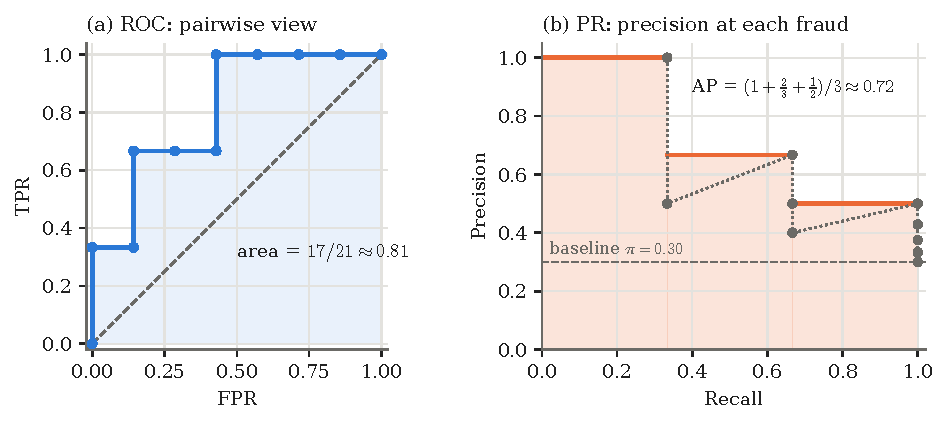
\includegraphics[width=\linewidth]{figs/fig_toy.pdf}
\caption{Toy example. (a) The shaded area under the ROC staircase is $17/21$. (b) $\AP$ is the
recall-weighted sum of the precision at each fraud; the shaded steps have widths $1/3$ and heights
$1$, $2/3$, $1/2$. Grey dots are the precision at every rank.}
\label{fig:toy}
\end{figure}

\subsection{One classifier, increasing imbalance}
Take the Gaussian score model of Figure~\ref{fig:curves}: negatives score $\mathcal N(0,1)$ and positives
$\mathcal N(\mu,1)$ with $\mu=2$. Then $\AUROC=\Phi(\mu/\sqrt2)\approx0.921$. Keep the classifier
\emph{exactly fixed} and change only the prevalence $\pi$, equivalently the number of legitimate cases
the model has to sift through.

\begin{table}[h]
\centering
\small
\caption{The same classifier at four prevalences (Gaussian model, $\mu=2$; values by numerical
integration of $\int \Prec\,d\Rec$).}
\label{tab:sweep}
\begin{tabular}{@{}rrcccc@{}}
\toprule
Prevalence $\pi$ & $k=N/P$ & ROC-AUC & AUC-PR (AP) & Baseline ($=\pi$) & AP\,/\,$\pi$ \\
\midrule
0.5   & 1   & 0.921 & 0.922 & 0.5   & 1.8 \\
0.1   & 9   & 0.921 & 0.665 & 0.1   & 6.7 \\
0.01  & 99  & 0.921 & 0.269 & 0.01  & 26.9 \\
0.001 & 999 & 0.921 & 0.062 & 0.001 & 61.8 \\
\bottomrule
\end{tabular}
\end{table}

\begin{figure}[t]
\centering
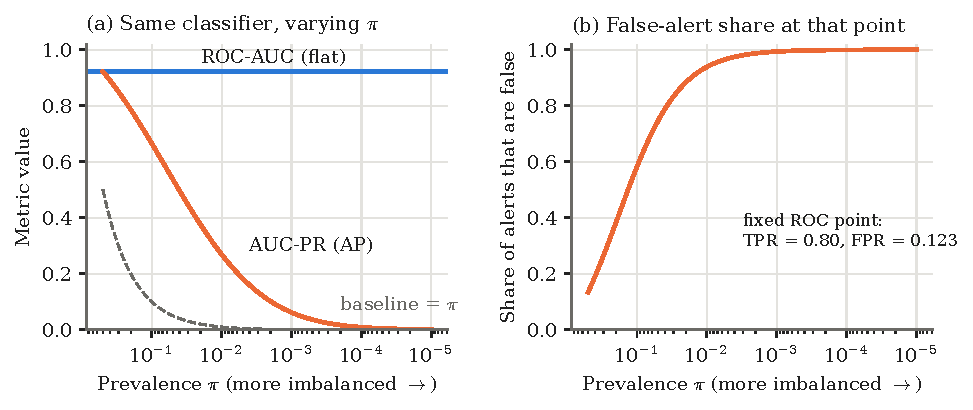
\includegraphics[width=\linewidth]{figs/fig_sweep.pdf}
\caption{(a) For a fixed classifier, ROC-AUC is flat in $\pi$ while AP falls toward zero. (b) Fix one
point on the ROC curve ($\TPR=0.80$, $\FPR=0.123$) and ask what share of the alerts raised there are
false alarms: $13\%$ at $\pi=0.5$, $58\%$ at $0.1$, $94\%$ at $0.01$, $99.4\%$ at $0.001$.}
\label{fig:sweep}
\end{figure}

\begin{proposition}[Negative inflation, a thought experiment]\label{prop:inflate}
Replace every negative case by $m$ copies drawn from the same distribution (so $N\to mN$ and
$k\to mk$). Then for every threshold $\TPR(t)$ and $\FPR(t)$ are unchanged, so the ROC curve and
ROC-AUC are \emph{exactly} unchanged, while $\mathrm{FP}\to m\,\mathrm{FP}$ and
$\Prec\to\TPR/(\TPR+mk\,\FPR)$, so the PR curve and $\AP$ change.
\end{proposition}
\begin{proof}
$\TPR$ conditions on positives, which were not touched; $\FPR=\Prob(S^{-}>t)$ is a probability under
the (unchanged) negative score distribution. Precision follows from Proposition~\ref{prop:bridge}
with $k$ replaced by $mk$.
\end{proof}

Going from $\pi=0.1$ to $\pi=0.01$ in Table~\ref{tab:sweep} is exactly this experiment with $m=11$:
the ROC-AUC does not move ($0.921$) while AP drops from $0.665$ to $0.269$.

\begin{remark}
These are population values. With a finite sample the estimate is noisy, especially when there are few
positives: a simulation with $10^6$ negatives and about $1000$ positives gave $\AP\approx0.057$ against
the population value $0.062$, whereas the ROC-AUC estimate ($\approx0.92$) is stable. Report confidence
intervals (e.g.\ by bootstrap) when $P$ is small.
\end{remark}

\subsection{Two models that ROC-AUC cannot tell apart}
Now compare two \emph{different} classifiers on a data set of $10^6$ transactions with $1000$ frauds
($\pi=0.001$, $k=999$). Model~A catches $60\%$ of the frauds while flagging only $0.1\%$ of legitimate
transactions; Model~B catches $80\%$ but flags $20\%$ of legitimate transactions. Interpolating linearly
to the corner $(1,1)$ gives the ROC curves in Figure~\ref{fig:models}(a).

\begin{table}[h]
\centering
\small
\caption{Models A and B at their first ROC vertex, and as summarised by the two areas ($k=999$).}
\label{tab:models}
\begin{tabular}{@{}lcccccc@{}}
\toprule
 & TPR & FPR & TP & FP & Precision & Alerts \\
\midrule
Model A & 0.60 & 0.001 & 600 & 999     & 0.375 & 1\,599 \\
Model B & 0.80 & 0.20  & 800 & 199\,800 & 0.004 & 200\,600 \\
\midrule
\multicolumn{7}{@{}l}{\textbf{ROC-AUC:} A $=0.7995$, \; B $=0.8000$ \quad (tied; B marginally ahead)}\\
\multicolumn{7}{@{}l}{\textbf{AUC-PR:} A $=0.227$, \; B $=0.0035$ \quad (A is $64\times$ better; baseline $=0.001$)}\\
\bottomrule
\end{tabular}
\end{table}

\begin{figure}[t]
\centering
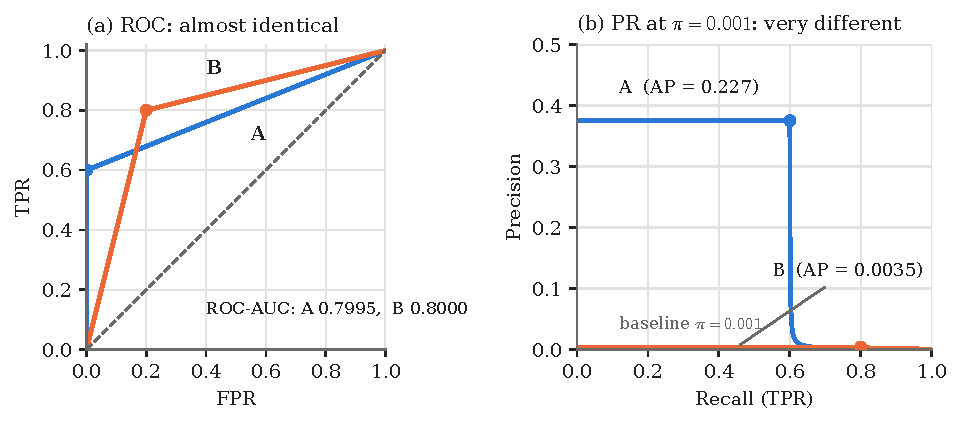
\includegraphics[width=\linewidth]{figs/fig_models.pdf}
\caption{(a) On the ROC plot the two models look equally good, with equal areas to three decimals.
Dots mark the first vertex of each curve. (b) At $\pi=0.001$ the PR curves are worlds apart: about one
alert in three is a real fraud for A, and about one in 250 for B.}
\label{fig:models}
\end{figure}

An investigation team would obviously prefer A. B finds a third more fraud but buries it under two
hundred times as many false alarms. ROC-AUC ranks B (marginally) first; AP ranks A first by a factor
of $64$. The analytic reason is the subject of the next section.

\subsection{What each metric is trying to accomplish}

\begin{center}
\small
\renewcommand{\arraystretch}{1.25}
\begin{tabular}{@{}p{3.1cm}p{5.7cm}p{5.7cm}@{}}
\toprule
 & \textbf{ROC-AUC} & \textbf{AUC-PR (AP)} \\
\midrule
Question it answers &
``If I draw a random fraud and a random legitimate case, how often is the fraud scored higher?'' &
``As I demand to catch more of the frauds, what fraction of my alerts are real?'' \\
Axes & $\TPR$ vs.\ $\FPR$ & Precision vs.\ recall \\
Uses true negatives & Yes (through $\FPR$) & No \\
Random baseline & $0.5$ & $\pi$ (prevalence) \\
Depends on $\pi$ & No (Theorem~\ref{thm:auc}) & Yes (through $k$; Section~4) \\
Cost of a false positive & Scaled by $1/N$: ignores how many negatives there are & Scaled by $k$: each false positive hurts more when negatives dominate \\
Where it looks & All FPR levels equally & The high-precision, low-FPR region \\
Best used when & Comparing rankers, or when the class ratio is unknown or will shift & Positives are rare and alerts are costly (fraud, screening, retrieval) \\
\bottomrule
\end{tabular}
\end{center}

\begin{insight}[Heuristic summary]
ROC-AUC measures \emph{ranking quality in a world where both classes are equally represented}; it is a
property of the two score distributions. AUC-PR measures \emph{usefulness of the alert list in the
world you will actually deploy in}: it bakes the class ratio into precision. When positives are rare,
that second question is the one that determines whether the model is useful, and
Proposition~\ref{prop:inflate} shows the first question cannot even see the difference.
\end{insight}

% =====================================================================
\section{Why AUC-PR is preferred under imbalance: a proof}
% =====================================================================

\subsection{Setting}
Parametrise the ROC curve by recall. Assume (for simplicity) that the ROC curve is the graph of a
continuous, nondecreasing function
\[
  g:[0,1]\to[0,1],\qquad g(r)=\FPR \text{ at the threshold where } \TPR=r,\qquad g(0)=0,\; g(1)=1 .
\]
(In general replace $g$ by a generalised inverse; the formulas hold as Stieltjes integrals.) Let
$r^{*}=\sup\{r:g(r)=0\}$ be the fraction of positives the model can capture before its first false alarm
($r^{*}=0$ for most real models). The data are described by the pair $(g,k)$: $g$ is a property of
the classifier, $k$ of the dataset.

\begin{lemma}[Both areas in terms of $g$]\label{lem:areas}
\[
  \AUROC \;=\; 1-\int_0^1 g(r)\,dr,
  \qquad\qquad
  \AP(k) \;=\; \int_0^1 \frac{r}{\,r+k\,g(r)\,}\,dr .
\]
\end{lemma}
\begin{proof}
The unit square is split by the ROC curve into the area under it, which is $\AUROC$, and the area to
its left, which is $\int_0^1 g(r)\,dr$ (integrating FPR against recall). The two add up to $1$. The AP
formula is $\int \Prec\,d\Rec$ with $\Prec=r/(r+k\,g(r))$ from Proposition~\ref{prop:bridge}.
\end{proof}

Lemma~\ref{lem:areas} is the whole argument in one line: \textbf{$k$ appears in AP and nowhere in
ROC-AUC.}

\subsection{ROC-AUC is blind to imbalance; AP is not}

\begin{theorem}[Behaviour of AP in $k$]\label{thm:ap}
For a fixed classifier (fixed $g$):
\begin{enumerate}[label=(\alph*)]
  \item \textbf{Monotonicity.} $\AP(k)$ is nonincreasing in $k$, and strictly decreasing whenever $g$ is not
        identically $0$. Indeed
        $\displaystyle \frac{\partial}{\partial k}\frac{r}{r+k\,g(r)}=-\frac{r\,g(r)}{(r+k\,g(r))^{2}}\le0 .$
  \item \textbf{Baseline.} For a no-skill classifier, $g(r)=r$, so $\AP=\int_0^1\frac{dr}{1+k}=\frac1{1+k}=\pi$.
  \item \textbf{Collapse.} $\displaystyle\lim_{k\to\infty}\AP(k)=r^{*}$. In particular $\AP\to0$ whenever the model
        cannot reach positive recall with zero false positives.
  \item \textbf{ROC-AUC is constant.} $\AUROC$ does not depend on $k$ (Lemma~\ref{lem:areas}).
\end{enumerate}
\end{theorem}
\begin{proof}
(a) is the derivative computation, integrated over $r$. (b) is direct substitution. For (c), the
integrand $r/(r+k\,g(r))$ is bounded by $1$ and, as $k\to\infty$, converges pointwise to $1$ on
$(0,r^{*})$ where $g=0$, and to $0$ on $(r^{*},1]$ where $g>0$ and $r>0$. By dominated convergence
$\AP(k)\to r^{*}$. (d) is Lemma~\ref{lem:areas}.
\end{proof}

So the same classifier has ROC-AUC fixed and AP sliding from near $1$ (balanced) down to $r^{*}$, which is
usually $0$, as the data become more imbalanced, exactly as in Table~\ref{tab:sweep}. AP is therefore
\emph{sensitive} to the quantity (the class ratio) that determines the real-world cost of false
alarms, while ROC-AUC is not.

\subsection{The two metrics look at different parts of the ROC curve}

Theorem~\ref{thm:ap} shows AP varies with $k$ but does not yet explain why that is the right behaviour,
nor how ROC-AUC could rank two models wrongly. The next result localises where each metric gets its
value.

\begin{theorem}[Complementary regions]\label{thm:regions}
Fix $\alpha\in(0,1)$.
\begin{enumerate}[label=(\roman*)]
  \item \textbf{ROC-AUC barely sees low FPR.} The part of ROC-AUC contributed by $\FPR\le\alpha$ is
        $\int_{0}^{\alpha}\TPR\,d\FPR\le\alpha$.
  \item \textbf{High precision lives at low FPR.} If $\Prec\ge p$ at recall $r$, then
        $g(r)\le \dfrac{(1-p)\,r}{p\,k}\le\dfrac{1-p}{p\,k}$. In particular $\Prec\ge\tfrac12$ forces
        $\FPR\le 1/k$.
  \item \textbf{AP barely sees high FPR.} The part of AP contributed by recall levels with
        $g(r)\ge\alpha$ is at most $\dfrac{1}{1+k\alpha}$.
\end{enumerate}
\end{theorem}
\begin{proof}
(i) $\TPR\le1$, so $\int_0^\alpha \TPR\,d\FPR\le\int_0^\alpha d\FPR=\alpha$.

(ii) $\Prec=r/(r+k\,g)\ge p$ rearranges to $g\le r(1-p)/(pk)$, and $r\le1$.

(iii) If $g(r)\ge\alpha$ then $\dfrac{r}{r+k\,g(r)}\le\dfrac{r}{r+k\alpha}\le\dfrac{1}{1+k\alpha}$, because
$r\mapsto r/(r+c)$ is increasing and $r\le1$. The set of such $r$ has measure at most $1$.
\end{proof}

\begin{corollary}[Disjoint supports under imbalance]\label{cor:regions}
Let $c>0$ and $\alpha=c/k$. Then
\[
  \underbrace{\text{ROC-AUC mass from } \FPR\le c/k}_{\le\; c/k}
  \qquad\text{while}\qquad
  \underbrace{\text{AP mass from } \FPR\ge c/k}_{\le\; 1/(1+c)} .
\]
For $\pi=0.001$ ($k=999$) and $c=9$: the region $\FPR\le0.9\%$ contributes at most $0.9\%$ of the area
to ROC-AUC, yet it carries all but at most $0.1$ of the value of AP.
\end{corollary}

In words: when $k$ is large, ROC-AUC is decided almost entirely by the part of the curve at
$\FPR>c/k$, where precision is already poor, and AP is decided almost entirely by the part at
$\FPR\le c/k$, which ROC-AUC essentially ignores. Only the second region is operationally affordable,
since an alert budget of $B$ false alarms means $\FPR\approx B/N=B/(kP)$.

\subsection{Ranking reversal: ROC-AUC can pick the wrong model}

Return to Models A and B of Section~3.3, with ROC curves through $(\FPR,\TPR)=(a,\rho)$ and linear
interpolation to $(1,1)$ ($a=0.001,\rho=0.6$ for A; $a=0.2,\rho=0.8$ for B), and $k=999$.

\textbf{ROC-AUC.} By the trapezoid rule, $\AUROC=\tfrac12 a\rho+\tfrac12(1-a)(1+\rho)$:
\[
  \AUROC_A=0.0003+0.7992=0.7995,\qquad
  \AUROC_B=0.08+0.72=0.8000 .
\]
\textbf{AP.} On the first segment $g(r)=ar/\rho$, so the integrand is the constant
$1/(1+ka/\rho)$ and the segment contributes
\[
  \rho\cdot\frac{1}{1+ka/\rho}=\frac{\rho^{2}}{\rho+ka}:\qquad
  A:\ \frac{0.36}{0.6+0.999}=0.2251,\qquad
  B:\ \frac{0.64}{0.8+199.8}=0.0032 .
\]
The second segment (from $\rho$ to $1$) adds $0.0017$ for A and $0.0004$ for B by numerical
integration, so
\[
  \AP_A\approx0.227,\qquad \AP_B\approx0.0035,\qquad \frac{\AP_A}{\AP_B}\approx64 .
\]

\textbf{Why this is not a coincidence.} Model~A's entire advantage over B lies in $\FPR\in[0,0.001]$. By
Theorem~\ref{thm:regions}(i) that slice can contribute at most $0.001$ to ROC-AUC (it contributes
$0.0003$), so B's lead of about $0.0008$ over the rest of the curve is enough to outweigh it. But by
Theorem~\ref{thm:regions}(ii) this slice is where precision can be as high as $\tfrac12$ or more, and
B has nothing there: its precision is $0.004$ at every point of its first segment and lower beyond it, so
$\AP_B<0.004$ however well it ranks in the high-FPR region. Any pair of models whose ROC curves differ
mainly at very low FPR can be reversed in the same way.

\subsection{Caveats and practical guidance}

\begin{itemize}
  \item \textbf{Same information, different weighting.} Davis and Goadrich showed that, on a fixed data set,
        one classifier's ROC curve dominates another's if and only if its PR curve does
        \cite{davis2006}. The two metrics differ because they \emph{integrate} different regions with
        different weights, not because one has information the other lacks.
  \item \textbf{ROC-AUC is not useless.} It is a valid, prevalence-free measure of ranking quality. It is the
        right tool when you want a property of the score distributions alone, or when the deployment
        class ratio is unknown or will shift. If you want to stay in ROC space under imbalance, use the
        \emph{partial} AUC restricted to $\FPR\le\alpha$.
  \item \textbf{AP is not comparable across data sets with different $\pi$.} Its baseline is $\pi$, so always
        report it with the baseline, or as lift $\AP/\pi$, or as the normalised
        $(\AP-\pi)/(1-\pi)$.
  \item \textbf{Pick the model by AP, the operating point by cost.} Use AUC-PR to choose between models, then
        choose the threshold from precision, recall and $\Fone$ (or $F_\beta$, or recall at a fixed alert
        budget) at the volume of alerts the investigation team can handle.
  \item \textbf{Mind the sample size.} AP estimated from few positives is noisy; use bootstrap intervals.
\end{itemize}

For an empirical treatment of the same point see Saito and Rehmsmeier \cite{saito2015}; for a general
introduction to ROC analysis see Fawcett \cite{fawcett2006}.

% =====================================================================
\begin{thebibliography}{9}
\bibitem{davis2006} J.~Davis and M.~Goadrich. The relationship between precision-recall and ROC curves.
  \emph{Proc.\ 23rd International Conference on Machine Learning (ICML)}, 233--240, 2006.
\bibitem{saito2015} T.~Saito and M.~Rehmsmeier. The precision-recall plot is more informative than the ROC
  plot when evaluating binary classifiers on imbalanced datasets. \emph{PLOS ONE}, 10(3):e0118432, 2015.
\bibitem{fawcett2006} T.~Fawcett. An introduction to ROC analysis. \emph{Pattern Recognition Letters},
  27(8):861--874, 2006.
\end{thebibliography}

\end{document}
